% !TEX program = pdflatex
\documentclass{article}

% ============================================================
%  NeurIPS 2026 Style
% ============================================================
\usepackage[final]{neurips_2026}   % camera-ready; use [preprint] for arXiv

% ============================================================
%  Packages
% ============================================================
\usepackage[T1]{fontenc}
\usepackage[utf8]{inputenc}
\usepackage{amsmath,amssymb,amsfonts,amsthm}
\usepackage{algorithmic}
\usepackage{algorithm}
\usepackage{booktabs}
\usepackage{multirow}
\usepackage{graphicx}
\usepackage{xcolor}
\usepackage{url}
\usepackage{hyperref}
\usepackage{bbm}
\usepackage{bm}
\usepackage{subcaption}
\usepackage{enumitem}
\usepackage{natbib}
\usepackage{microtype}
\usepackage{cleveref}

\hypersetup{
  colorlinks=true,
  linkcolor=blue!60!black,
  citecolor=blue!60!black,
  urlcolor=blue!70!black
}

\setlist{nosep}

% ============================================================
%  Theorem Environments
% ============================================================
\newtheorem{theorem}{Theorem}
\newtheorem{lemma}[theorem]{Lemma}
\newtheorem{corollary}[theorem]{Corollary}
\newtheorem{proposition}[theorem]{Proposition}
\newtheorem{definition}[theorem]{Definition}
\newtheorem{remark}[theorem]{Remark}

% ============================================================
%  Custom Commands
% ============================================================
\newcommand{\ie}{\textit{i.e.}}
\newcommand{\eg}{\textit{e.g.}}
\newcommand{\etal}{\textit{et al.}}
\newcommand{\wrt}{w.r.t.}
\newcommand{\UDL}{\mathrm{UDL}}
\newcommand{\R}{\mathbb{R}}
\newcommand{\E}{\mathbb{E}}
\newcommand{\Nset}{\mathcal{S}}  % Normal set (avoid \mathcal{N} ≈ Gaussian confusion)
\newcommand{\T}{\mathcal{T}}
\newcommand{\calR}{\mathcal{R}}
\newcommand{\norm}[1]{\left\lVert#1\right\rVert}
\newcommand{\abs}[1]{\left\lvert#1\right\rvert}
\DeclareMathOperator{\erf}{erf}
\DeclareMathOperator{\tr}{tr}
\DeclareMathOperator{\rank}{rank}
\DeclareMathOperator{\diag}{diag}
\DeclareMathOperator*{\argmax}{arg\,max}
\DeclareMathOperator*{\argmin}{arg\,min}

% ============================================================
%  Title
% ============================================================
\title{The Universal Deviation Principle: Multi-Spectrum Sensitivity Guarantees\\for Anomaly Detection}

\author{
  Odeyemi Olusegun Israel \\
  Independent Researcher \\
  \texttt{segettii@gmail.com} \\
  ORCID: \href{https://orcid.org/0009-0004-2309-6436}{0009-0004-2309-6436}
}

\begin{document}
\maketitle

% ============================================================
%  Abstract
% ============================================================
\begin{abstract}
We introduce the \textbf{Universal Deviation Principle (UDP)}, a theoretically grounded framework for multi-perspective anomaly detection. The core principle is that, under explicit assumptions on operator-family richness and anomaly-normal separation in feature space, a point which is \emph{meaningfully different from the normal set} cannot simultaneously match normality under all structural perspectives. We formalise this via \emph{deviation-separating operator families}, collections of differentiable maps $\{\Phi_k\}_{k=1}^K$ whose stacked Jacobian has full column rank, yielding local distinguishability around a reference normal state $\bm{\mu}$. To connect the sensitivity theory to detection, we define a normal set $\Nset$ and a deviation score based on distance of $\Phi(\mathbf{x})$ to $\Phi(\Nset)$; under an explicit separation condition between normal and anomaly sets in operator space, at least one operator deviates by a positive margin. All theoretical results are conditional on three stated assumptions (observability, operator-family richness, calibration discipline). We prove five results: (1)~local distinguishability via the Inverse Function Theorem; (2)~global sensitivity via compactness and the Extreme Value Theorem with a uniform bound $\underline{\sigma} > 0$; (3)~finite-sample guarantees via Hoeffding concentration; (4)~fusion weights maximising worst-case directional sensitivity via a semidefinite programme; and (5)~a greedy operator selection algorithm with $(1-1/e)$-approximation guarantee via monotone submodularity. We instantiate the framework with five spectrum projection operators (statistical, dynamical, spectral, geometric, exponential) and introduce a \textbf{Boundary-Centred Dimension Magnifier} paired with QDA that, given labels, achieves strong supervised performance. The unsupervised MDN score provides a label-free alternative (mean AUC $0.829$ across five benchmarks).

We also present the \textbf{GravityEngine}, an N-body scoring algorithm whose force potentials we derive in closed form. The attraction potential involves the error function $\erf(r/\sigma)$. With backtracking line-search, the energy decreases monotonically at every observed iteration; the descent guarantee holds conditional on the line-search finding a step within the halving budget. Beyond the 5~base operators, we extend the framework to 14~composable spectrum operators across five mathematical families. A correlation audit across all 91~operator pairs reveals only one redundant pair (Wavelet$\leftrightarrow$Phase, $\rho{=}0.92$), validating the multi-spectrum thesis. We introduce \textbf{top-$k$ coverage} as a complementary metric to AUC, revealing failure modes where high AUC does not translate to actionable detection. UDL-Hybrid with auto-selected projection strategy achieves mean AUC $0.972$ and 91\% mean coverage across five benchmarks, \textbf{exceeding all established baselines}. GravityEngine reaches AUC $0.899$ on mammography with empirically verified monotone energy decrease (14/14 iteration steps). We numerically verify the theorem conditions on three independent ODDS benchmarks via Monte Carlo checks and observe no violations in our samples. Code is available at \url{https://github.com/segetii/fintech}.
\end{abstract}

% ============================================================
%  1. Introduction
% ============================================================
\section{Introduction}
\label{sec:introduction}

Every anomaly detector makes assumptions about what anomalies look like. Isolation Forest \citep{liu2008isolation} assumes geometric isolation. LOF \citep{breunig2000lof} assumes local density deviation. Deep SVDD \citep{ruff2018deep} assumes separation from a learned hypersphere. Each works well when its assumptions hold, and each has blind spots when they do not. An anomaly that mimics normal local density will evade LOF entirely, yet the same anomaly may be obvious under spectral analysis or geometric projection. This is not a minor inconvenience; it is a structural limitation that recurs across fraud detection \citep{ahmed2016survey}, medical diagnosis \citep{fernando2021deep}, cybersecurity \citep{chandola2009anomaly}, industrial monitoring \citep{pang2021deep}, and aerospace telemetry \citep{hundman2018detecting}.

A natural question follows: can we state conditions under which combining multiple mathematical perspectives makes anomalies detectable? This paper answers in the affirmative under explicit assumptions on operator-family richness, feature observability, and calibration discipline. We introduce the \textbf{Universal Deviation Principle (UDP)}, which provides local, global, finite-sample, and algorithmic guarantees for operator-family sensitivity, and a set-based separation condition that turns sensitivity into a detection statement. All theoretical results are conditional on these assumptions; we state them explicitly in \Cref{sec:theory}.

\textbf{Contributions.} Our contributions are:
\begin{enumerate}[leftmargin=*]
    \item \textbf{Theoretical framework} (\Cref{sec:theory}): Three explicit assumptions (observability, operator-family richness, calibration discipline) under which five conditional results establish \emph{sensitivity/distinguishability} for deviation-separating operator families, plus an explicit set-based separation condition that yields a detection guarantee. This includes local (\Cref{thm:local}) and global (\Cref{thm:global}) sensitivity bounds, finite-sample bounds (\Cref{thm:finite}), fusion weights maximising worst-case sensitivity via SDP (\Cref{thm:sdp}), and greedy selection with $(1-1/e)$-approximation (\Cref{thm:greedy}). The individual proof techniques (IFT, EVT, Hoeffding, SDP relaxation, submodular optimisation) are classical; the contribution is the \emph{framework} that threads them into end-to-end conditions for detectability.
    \item \textbf{GravityEngine} (\Cref{sec:gravity}): An N-body scoring algorithm with a closed-form energy functional (attraction via $\erf$ potential, logarithmic repulsion, quadratic confinement). Backtracking line-search yields monotone energy descent at every observed iteration (\Cref{thm:lyapunov}); we state the descent guarantee conditional on the line-search finding a step within the halving budget.
    \item \textbf{Multi-spectrum architecture} (\Cref{sec:framework}): Five composable spectrum operators, a Boundary-Centred Dimension Magnifier with saturating $\tanh$ non-linearity, and QDA-Magnified projection achieving state-of-the-art AUC.
    \item \textbf{Empirical evaluation} (\Cref{sec:experiments}): Five datasets across four domains, a single hyperparameter set throughout, comparisons against seven baselines including Deep SVDD and ECOD, 5-fold cross-validation on mammography, per-law decomposition analysis (including pendigits), and numerical checks of theorem conditions on three ODDS datasets.
\end{enumerate}

% ============================================================
%  2. Related Work
% ============================================================
\section{Related Work}
\label{sec:related}

\textbf{Classical methods.} Distance-based approaches ($k$-NN \citep{ramaswamy2000efficient}, Mahalanobis) and density-based methods (LOF \citep{breunig2000lof}, DBSCAN \citep{ester1996density}) operate in geometric space. Tree-based methods like Isolation Forest \citep{liu2008isolation} exploit random partitioning. All of these impose a single mathematical viewpoint on the data.

\textbf{Deep approaches.} Autoencoder-based detectors \citep{an2015variational,zhou2017anomaly} flag high reconstruction error. Deep SVDD \citep{ruff2018deep} learns a minimum-volume hypersphere. GANs \citep{schlegl2017unsupervised} model the normal distribution and flag deviations from it. These capture complex patterns, but they still produce a single representation of normality.

\textbf{Modern unsupervised detectors.} ECOD \citep{li2022ecod} uses empirical cumulative distribution functions per feature. COPOD \citep{li2020copod} extends this with copula-based dependence modelling. Both achieve competitive performance in $O(n)$ time. Neither provides theoretical detectability guarantees.

\textbf{OOD detection.} Hendrycks and Gimpel~\citep{hendrycks2017baseline} showed that softmax probabilities give a usable OOD baseline; ODIN \citep{liang2018odin} and energy-based methods \citep{liu2020energy} improved on it. These produce a single OOD score. UDL differs because it decomposes \emph{which mathematical aspect} makes an observation anomalous.

\textbf{Ensemble and multi-view methods.} Feature bagging \citep{lazarevic2005feature} and detector aggregation \citep{aggarwal2015theoretical} combine multiple instances of similar detectors. Krogh and Vedelsby~\citep{krogh1995neural} proved that ensemble error decreases with member diversity. UDL's diversity operates at the \emph{representation} level rather than the \emph{model} level: it fuses mathematically distinct projection operators, not multiple copies of the same detector.

\textbf{Physics-inspired clustering.} Particle swarm optimisation \citep{kennedy1995particle}, gravitational search \citep{rashedi2009gsa}, and charged system search \citep{kaveh2010css} use physical analogies for optimisation. GravityEngine differs in two ways: its potential functions are derived from the force field in closed form with force-energy consistency ($F = -\nabla E$) verified analytically, and backtracking line-search enforces monotone energy descent at every observed iteration.

\textbf{Benchmarking.} PyOD \citep{zhao2019pyod} implements over 30 detectors. ADBench \citep{han2022adbench} provides 57 benchmark datasets. We evaluate on ODDS benchmarks \citep{rayana2016odds} and follow ADBench protocols.

% ============================================================
%  3. Theory: Universal Deviation Law
% ============================================================
\section{Universal Deviation Principle: Theory}
\label{sec:theory}

\subsection{Scope and Assumptions}

The theoretical results in this section are conditional on three explicit assumptions. We state them upfront so that the scope of each theorem is unambiguous.

\begin{description}[leftmargin=*,labelwidth=1.8cm]
\item[A1 (Observability)] Anomalies are detectable from available features: the anomaly definition is \emph{feature-realisable}, meaning there exists a measurable difference between normal and anomalous observations in $\R^d$. This excludes ``label-only'' anomalies where $\mathbf{x} \in \mathrm{supp}(P_{\text{normal}})$ but the label is adverse for reasons invisible in the feature space.
\item[A2 (Operator-family richness)] For any $\mathbf{x}$ that violates a normal model (see A1), there exists at least one operator $\Phi_k$ in the family for which the induced deviation exceeds a positive margin. Formally, the stacked Jacobian has full column rank (\Cref{def:separating}), and the separation condition of \Cref{thm:separation} holds with $\Delta > 0$. This assumption can fail if operators are redundant or insensitive on certain subspaces; we verify it empirically via Monte Carlo checks (\Cref{tab:theorem_verification}).
\item[A3 (Calibration discipline)] All operator statistics, thresholds, and fusion weights are estimated on normal training data only. No test-set information (labels, statistics, or thresholds) is used in any step of score computation, operator selection, or decision boundary calibration.
\end{description}

\textbf{What these assumptions exclude.} A1 excludes adversarial label anomalies where $\mathbf{x}$ is indistinguishable from normals in feature space. A2 excludes degenerate operator families (e.g., $K$ copies of the same linear projection). A3 excludes any form of test-set leakage. When all three hold, the theorems below provide conditional guarantees. When they do not, the framework reduces to an empirical multi-view anomaly detector with no formal guarantees---still useful, but not ``proved.''

\subsection{Deviation-Separating Operator Families}

\begin{definition}[Deviation-Separating Family]
\label{def:separating}
Let $\{\Phi_k\}_{k=1}^K$, $\Phi_k: \R^d \to \R^{d_k}$, be continuously differentiable operators. The family is \emph{deviation-separating at $\bm{\mu} \in \R^d$} if:
\begin{equation}
\bigcap_{k=1}^{K} \ker\!\left(D\Phi_k(\bm{\mu})\right) = \{\mathbf{0}\}
\label{eq:separating}
\end{equation}
Equivalently (\Cref{lem:rank}), the stacked Jacobian $J(\bm{\mu}) = [D\Phi_1(\bm{\mu})^\top, \ldots, D\Phi_K(\bm{\mu})^\top]^\top \in \R^{D \times d}$ has full column rank, where $D = \sum_k d_k$.
\end{definition}

\begin{lemma}[Rank Characterisation]
\label{lem:rank}
$\{\Phi_k\}$ is deviation-separating at $\bm{\mu}$ if and only if $\rank(J(\bm{\mu})) = d$.
\end{lemma}

The proof is immediate: $\ker(J(\bm{\mu})) = \bigcap_k \ker(D\Phi_k(\bm{\mu}))$.

\subsection{From Sensitivity to Detection: A Normal Set $\Nset$}

Theorems~\ref{thm:local}--\ref{thm:finite} are sensitivity statements around a reference point $\bm{\mu}$: they guarantee that \emph{any} perturbation away from $\bm{\mu}$ produces a response in at least one operator under rank conditions. To interpret this as anomaly detection, we must specify what ``normal'' means (a set or distribution) and a detection statistic.

\begin{definition}[Normal Set and Deviation Score]
\label{def:normal_set}
Let $\Nset \subset \R^d$ denote the set of normal states (e.g., the support of a normal distribution $P_\Nset$ or an empirical normal training set). Define the joint operator map $\Phi(\mathbf{x}) := (\Phi_1(\mathbf{x}),\ldots,\Phi_K(\mathbf{x})) \in \R^{D}$, $D=\sum_k d_k$. Define the set-distance deviation score
\begin{equation}
s_\Nset(\mathbf{x}) := \mathrm{dist}(\Phi(\mathbf{x}),\Phi(\Nset)) = \inf_{\mathbf{z}\in \Nset}\, \norm{\Phi(\mathbf{x})-\Phi(\mathbf{z})}_2.
\label{eq:set_score}
\end{equation}
For per-operator analysis, define $s_{\Nset,k}(\mathbf{x}) := \mathrm{dist}(\Phi_k(\mathbf{x}),\Phi_k(\Nset))$.
\end{definition}

\begin{theorem}[Separation in Operator Space Implies Detectability]
\label{thm:separation}
Assume $\Nset$ is compact and each $\Phi_k$ is continuous. Let $\mathcal{A}\subset\R^d$ be a compact set of anomalies with $\mathcal{A}\cap \Nset=\emptyset$, and assume there exists a margin $\Delta>0$ such that
\begin{equation}
\mathrm{dist}(\Phi(\mathcal{A}),\Phi(\Nset)) \ge \Delta.
\label{eq:operator_separation}
\end{equation}
Then for all $\mathbf{x}\in\mathcal{A}$, $s_\Nset(\mathbf{x})\ge \Delta$ and in particular there exists $k\in\{1,\ldots,K\}$ such that
\begin{equation}
s_{\Nset,k}(\mathbf{x}) \ge \Delta/\sqrt{K}.
\end{equation}
\end{theorem}

\begin{remark}[What the guarantee does and does not claim]
\label{rem:detection_scope}
The separation condition~\eqref{eq:operator_separation} is an explicit modelling assumption: if anomalies are not separated from normals in operator space (e.g., an adversary constructs $\mathbf{x}\notin\Nset$ with $\Phi(\mathbf{x})\in\Phi(\Nset)$), no operator-based detector can succeed. UDL provides (i) conditions under which perturbations are not invisible (rank conditions), and (ii) a clean separation-to-detection statement once a normal set $\Nset$ and a detection score are fixed.
\end{remark}

\textbf{Empirical evidence for operator-space separation.} To verify that the separation assumption $\Delta > 0$ holds in practice, we compute Cohen's $d$ (standardised centroid distance) between anomaly and normal embeddings $\Phi(\mathcal{A})$, $\Phi(\Nset)$ on all five benchmarks. The empirical values are: Synthetic $d=14.6$, Mimic $d=13.7$, Mammography $d=3.3$, Shuttle $d=0.43$, Pendigits $d=0.81$. All are strictly positive, confirming that the joint operator map induces measurable separation on every dataset. The variation across datasets reflects detection difficulty: large $d$ (synthetic, mimic) corresponds to trivial detection (AUC $\approx 1.0$), while smaller $d$ (shuttle, pendigits) correlates with harder tasks. Per-law analysis shows the geometric spectrum contributes the largest separation on four of five datasets, consistent with the per-law AUC results in \Cref{tab:perlaw}.

\subsection{Main Theorems}

\begin{theorem}[Universal Deviation, Local Form]
\label{thm:local}
Let $\{\Phi_k\}_{k=1}^K$ be a deviation-separating family at $\bm{\mu}$ with each $\Phi_k \in C^1$. Then there exists an open neighbourhood $U \ni \bm{\mu}$ such that for every $\mathbf{x} \in U \setminus \{\bm{\mu}\}$:
\begin{equation}
\exists\, k \in \{1,\ldots,K\}: \quad \Phi_k(\mathbf{x}) \neq \Phi_k(\bm{\mu})
\end{equation}
Since $J(\bm{\mu})$ has full column rank and singular values depend continuously on the matrix, there exists $\varepsilon > 0$ such that $\rank(J(\mathbf{x})) = d$ for all $\mathbf{x} \in B(\bm{\mu}, \varepsilon)$. This neighbourhood is precisely the $U$ above.

With $\sigma_{\min} := \sigma_{\min}(J(\bm{\mu})) > 0$, a quantitative bound holds:
\begin{equation}
\max_{k} \norm{\Phi_k(\mathbf{x}) - \Phi_k(\bm{\mu})} \geq \frac{\sigma_{\min}}{\sqrt{K}} \norm{\mathbf{x} - \bm{\mu}} - O(\norm{\mathbf{x} - \bm{\mu}}^2)
\label{eq:quantitative}
\end{equation}
\end{theorem}

\begin{theorem}[Universal Deviation, Global Form]
\label{thm:global}
Let each $\Phi_k \in C^2$, and let $\mathcal{K} \subset \R^d$ be compact with $\rank(J(\mathbf{x})) = d$ for all $\mathbf{x} \in \mathcal{K}$. Define
$\underline{\sigma} := \min_{\mathbf{x} \in \mathcal{K}} \sigma_{\min}(J(\mathbf{x}))$.
Then $\underline{\sigma} > 0$, and for all $\mathbf{x} \in \mathcal{K}$:
\begin{equation}
\max_{k} \norm{\Phi_k(\mathbf{x}) - \Phi_k(\bm{\mu})} \geq \frac{\underline{\sigma}}{\sqrt{K}} \norm{\mathbf{x} - \bm{\mu}} - C\norm{\mathbf{x} - \bm{\mu}}^2
\label{eq:global}
\end{equation}
where $C = \frac{1}{2}\sup_{\mathbf{z} \in \mathcal{K}} \norm{D^2\Phi(\mathbf{z})}$ is finite by continuity of $D^2\Phi$ on the compact set.
\end{theorem}

\begin{theorem}[Finite-Sample Deviation Guarantee]
\label{thm:finite}
Let $\hat{\bm{\mu}}_n = \frac{1}{n}\sum_{i=1}^n \mathbf{x}_i$ with $\mathbf{x}_i \overset{\text{iid}}{\sim} P_\Nset$ sub-Gaussian, population mean $\bm{\mu}$, covariance $\Sigma$. Let each $\Phi_k$ be $L_k$-Lipschitz, $L = \max_k L_k$. Then with probability $\geq 1 - \delta$:
\begin{equation}
\max_{k} \norm{\Phi_k(\mathbf{x}) - \Phi_k(\hat{\bm{\mu}}_n)} \geq \frac{\underline{\sigma}}{\sqrt{K}}\norm{\mathbf{x} - \bm{\mu}} - \frac{L\sqrt{\tr(\Sigma)}\sqrt{2\ln(2d/\delta)}}{\sqrt{n}}
\label{eq:finite}
\end{equation}
\end{theorem}

\begin{corollary}[Sample Complexity]
\label{cor:sample}
The bound~\eqref{eq:finite} is non-trivial when $n > 2L^2 K \cdot \tr(\Sigma) \cdot \ln(2d/\delta) / (\underline{\sigma}^2 \norm{\mathbf{x}-\bm{\mu}}^2)$.
\end{corollary}

\begin{theorem}[Worst-Case Sensitivity Maximisation via SDP]
\label{thm:sdp}
Define per-operator information matrices $\mathcal{I}_k := D\Phi_k(\bm{\mu})^\top D\Phi_k(\bm{\mu}) \succeq 0$. The worst-case detection sensitivity under weighted fusion $S_\mathbf{w}[\mathbf{x}] = \sum_k w_k \|\Phi_k(\mathbf{x}) - \Phi_k(\bm{\mu})\|^2$ is:
\begin{equation}
\eta(\mathbf{w}) := \lambda_{\min}\!\left(\textstyle\sum_k w_k \mathcal{I}_k\right)
\end{equation}
which is concave on the simplex $\Delta_K$ (since $\lambda_{\min}$ is an infimum of linear functions). Geometrically, $\eta(\mathbf{w})$ is the worst-case directional sensitivity: the minimum squared response of the fused operator to any unit perturbation. Maximising $\eta$ over $\mathbf{w} \in \Delta_K$ yields the weight vector $\mathbf{w}^*$ that makes the weakest detection direction as strong as possible, solvable as a standard SDP.
\end{theorem}

\begin{remark}[Finite-sample caveat for SDP weights]
\label{rem:sdp_estimation}
The SDP uses $\mathcal{I}_k$ matrices computed from $D\Phi_k(\bm{\mu})$, which in practice is estimated from data via finite differences. The ``optimality'' of $\mathbf{w}^*$ is therefore only as good as the Jacobian estimates; under finite-sample estimation noise, the true worst-case sensitivity may differ. We treat the SDP as a principled optimisation heuristic with population-level optimality, not a finite-sample guarantee, and verify empirically that SDP weights outperform equal weights on two of three datasets (\Cref{tab:theorem_verification}).
\end{remark}

\begin{theorem}[Greedy Operator Selection]
\label{thm:greedy}
Given $M$ candidate operators with $\mathcal{I}_k \succeq 0$ for each $k$ and budget $K$, selecting $S^*$ to maximise $\lambda_{\min}(\sum_{k \in S} \mathcal{I}_k)$ is NP-hard. The surrogate $f(S) = \log\det(\sum_{k \in S} \mathcal{I}_k)$ is monotone submodular (monotonicity and diminishing returns both require $\mathcal{I}_k \succeq 0$), and greedy selection achieves:
\begin{equation}
f(S_{\text{greedy}}) \geq (1 - 1/e) \cdot f(S^*)
\end{equation}
\end{theorem}

\textbf{Surrogate gap.} The $(1-1/e)$ guarantee holds for $f(S) = \log\det(\cdot)$, not directly for $\lambda_{\min}(\cdot)$. In practice the two objectives are correlated: maximising the log-determinant tends to raise the smallest eigenvalue because $\log\det = \sum \log\lambda_i$ penalises small eigenvalues logarithmically. Bounding the gap between the two objectives in the worst case remains open; we report both SDP-optimal and greedy performance empirically (\Cref{tab:theorem_verification}).

All proofs are in \Cref{app:proofs}.

\subsection{How $J(\mathbf{x})$ is computed in practice}
\label{ssec:jacobian_practice}
For general (nonlinear) operators where analytic derivatives are inconvenient, we estimate each Jacobian $D\Phi_k(\bm{\mu})$ by central finite differences. Concretely, for input dimension $d$ and reference point $\bm{\mu}$, we perturb coordinate $j$ by $\varepsilon_j=\varepsilon(\abs{\mu_j}+10^{-6})$ and compute
\begin{equation}
\frac{\partial \Phi_k}{\partial x_j}(\bm{\mu}) \approx \frac{\Phi_k(\bm{\mu}+\varepsilon_j\mathbf{e}_j)-\Phi_k(\bm{\mu}-\varepsilon_j\mathbf{e}_j)}{2\varepsilon_j}.
\end{equation}
We then stack the per-operator Jacobians vertically to form $J(\bm{\mu})$ and compute $\sigma_{\min}(J)$ via SVD. This matches the implementation used in our operator-diversity diagnostics (see the finite-difference Jacobian routine in \texttt{udl/energy.py}).

% ============================================================
%  4. GravityEngine: N-Body Variational Scoring
% ============================================================
\section{GravityEngine: N-Body Variational Scoring}
\label{sec:gravity}

The theoretical framework of \Cref{sec:theory} provides sensitivity/distinguishability guarantees conditional on Assumptions A1--A3 and, under the explicit separation condition of Theorem~\ref{thm:separation}, a detectability statement. We now turn to the question of \emph{how to score} observations. The GravityEngine implements the deviation principle through energy-inspired N-body dynamics.

\subsection{Force Field}

Each data point $\mathbf{x}_i$ is treated as a particle subject to three forces:

\textbf{Radial anchoring.} A spring-like restoring force toward the data centroid:
\begin{equation}
\mathbf{F}_{\text{radial}}(\mathbf{x}_i) = -\alpha(\mathbf{x}_i - \bm{\mu})
\label{eq:f_radial}
\end{equation}

\textbf{Pairwise interaction.} Short-range attraction with close-range repulsion between particles:
\begin{equation}
\mathbf{F}_{\text{pair}}(\mathbf{x}_i) = -\gamma \sum_{j \neq i} \left[\exp\!\left(-\frac{r_{ij}^2}{\sigma^2}\right) - \frac{\lambda}{r_{ij}}\right] \hat{\mathbf{r}}_{ij}
\label{eq:f_pair}
\end{equation}
where $r_{ij} = \norm{\mathbf{x}_i - \mathbf{x}_j}$ and $\hat{\mathbf{r}}_{ij}$ is the unit vector from $j$ to $i$.

\textbf{Deviation penalty.} Connects to the UDL framework via the quadratic operator $\Phi(\mathbf{x}) = \mathbf{x}^2$. The deviation energy is $V_{\text{dev}} = \frac{\beta}{2}\norm{\mathbf{x}^2 - \bm{\mu}^2}^2$; the force is its negative gradient:
\begin{equation}
F_{\text{dev},j}(\mathbf{x}_i) = -\frac{\partial V_{\text{dev}}}{\partial x_{ij}} = -2\beta\, x_{ij}(x_{ij}^2 - \mu_j^2)
\label{eq:f_dev}
\end{equation}
i.e.\ $\mathbf{F}_{\text{dev}} = -2\beta\,\mathbf{x}_i \odot (\mathbf{x}_i^2 - \bm{\mu}^2)$, where $\odot$ is the Hadamard product.

After iterative evolution, normal points cluster together. Anomalies do not. They end up in isolated positions. The anomaly score is simply the displacement $\norm{\mathbf{x}_i^{(\text{final})} - \mathbf{x}_i^{(\text{initial})}}$.

\subsection{Deriving the Correct Energy Functional}

For the energy functional to serve as a descent objective, the forces must satisfy $\mathbf{F} = -\nabla E$. If the energy and forces are inconsistent, the system is not performing gradient descent on any well-defined functional, and monotone-descent claims cannot be made. We derive each potential by integration:

\textbf{Radial potential.} From $\mathbf{F} = -\alpha(\mathbf{x} - \bm{\mu})$:
\begin{equation}
V_{\text{radial}}(\mathbf{x}) = \frac{\alpha}{2}\norm{\mathbf{x} - \bm{\mu}}^2
\label{eq:v_radial}
\end{equation}

\textbf{Pairwise attraction potential.} The radial force magnitude from attraction is $f_a(r) = \gamma\exp(-r^2/\sigma^2)$. We need $V_a(r)$ such that $dV_a/dr = f_a(r)$:
\begin{equation}
V_{\text{attract}}(r) = \gamma \int_0^r \exp\!\left(-\frac{s^2}{\sigma^2}\right) ds = \gamma \cdot \frac{\sigma\sqrt{\pi}}{2} \cdot \erf\!\left(\frac{r}{\sigma}\right)
\label{eq:v_attract}
\end{equation}
where $\erf(z) = \frac{2}{\sqrt{\pi}}\int_0^z e^{-t^2} dt$ is the error function.

\textbf{Verification:} $\frac{d}{dr}\!\left[\gamma\frac{\sigma\sqrt{\pi}}{2}\erf(r/\sigma)\right] = \gamma\frac{\sigma\sqrt{\pi}}{2} \cdot \frac{2}{\sigma\sqrt{\pi}} e^{-r^2/\sigma^2} = \gamma e^{-r^2/\sigma^2}$. \checkmark

\textbf{Pairwise repulsion potential.} From $f_r(r) = -\gamma\lambda/r$:
\begin{equation}
V_{\text{repel}}(r) = -\gamma\lambda \ln r
\label{eq:v_repel}
\end{equation}

\textbf{Deviation potential.} From $F_j = -2\beta\, x_j(x_j^2 - \mu_j^2)$, we need $V$ with $\partial V/\partial x_j = 2\beta\, x_j(x_j^2 - \mu_j^2)$. Noting $\frac{\partial}{\partial x_j}\!\left[\frac{1}{2}(x_j^2 - \mu_j^2)^2\right] = 2x_j(x_j^2 - \mu_j^2)$:
\begin{equation}
V_{\text{dev}}(\mathbf{x}) = \frac{\beta}{2}\norm{\mathbf{x}^2 - \bm{\mu}^2}^2
\label{eq:v_dev}
\end{equation}
\textbf{Verification:} $\frac{\partial V_{\text{dev}}}{\partial x_j} = \beta(x_j^2 - \mu_j^2) \cdot 2x_j = 2\beta\, x_j(x_j^2 - \mu_j^2)$. \checkmark

The total energy is:
\begin{equation}
\boxed{
E(\mathbf{X}) = \frac{\alpha}{2}\sum_i \norm{\mathbf{x}_i - \bm{\mu}}^2 + \gamma\frac{\sigma\sqrt{\pi}}{2}\sum_{i<j}\erf\!\left(\frac{r_{ij}}{\sigma}\right) - \gamma\lambda\sum_{i<j}\ln r_{ij} + \frac{\beta}{2}\sum_i \norm{\mathbf{x}_i^2 - \bm{\mu}^2}^2
}
\label{eq:energy}
\end{equation}

\subsection{Monotone Convergence via Backtracking Line-Search}

Discrete Euler integration $\mathbf{X}^{t+1} = \mathbf{X}^t + \eta \mathbf{F}(\mathbf{X}^t)$ can overshoot and increase energy when $\eta$ is too large. A fixed step size would require theoretical bounds on the Lipschitz constant of $\nabla E$, which are hard to obtain for an N-body system. Backtracking line-search (\Cref{alg:linesearch}) avoids this problem entirely by checking the energy at each step and halving $\eta$ until descent is achieved.

\begin{algorithm}[t]
\caption{GravityEngine Iteration with Backtracking Line-Search}
\label{alg:linesearch}
\begin{algorithmic}[1]
\REQUIRE Data $\mathbf{X}^0$, learning rate $\eta$, damping $\rho \in (0,1]$, shrink factor $\beta_{\text{ls}} \in (0,1)$, max halvings $L$
\FOR{$t = 0, 1, \ldots, T-1$}
    \STATE $\mathbf{F} \leftarrow -\nabla E(\mathbf{X}^t)$ \hfill $\triangleright$ Total force
    \STATE $\eta_t \leftarrow \eta$ \hfill $\triangleright$ Initial step size
    \FOR{$\ell = 0, 1, \ldots, L-1$}
        \STATE $\mathbf{X}_{\text{trial}} \leftarrow \mathbf{X}^t + \eta_t \cdot \rho \cdot \mathbf{F}$
        \IF{$E(\mathbf{X}_{\text{trial}}) \leq E(\mathbf{X}^t)$}
            \STATE $\mathbf{X}^{t+1} \leftarrow \mathbf{X}_{\text{trial}}$; \textbf{break}
        \ELSE
            \STATE $\eta_t \leftarrow \beta_{\text{ls}} \cdot \eta_t$ \hfill $\triangleright$ Halve step
        \ENDIF
    \ENDFOR
\ENDFOR
\RETURN $\mathbf{X}^T$
\end{algorithmic}
\end{algorithm}

\begin{proposition}[Conditional Monotone Energy Descent]
\label{thm:lyapunov}
Let $E$ be defined by~\eqref{eq:energy} with $\alpha > 0$, and let $\mathbf{X}^{t+1}$ be obtained from $\mathbf{X}^t$ by \Cref{alg:linesearch}. Assume the line-search finds a step $\eta_t > 0$ satisfying $E(\mathbf{X}^{t+1}) \leq E(\mathbf{X}^t)$ within $L$ halvings (i.e., the halving budget is sufficient). Then:
\begin{equation}
E(\mathbf{X}^{t+1}) \leq E(\mathbf{X}^t) \quad \text{for all $t$ where the line-search succeeds}
\end{equation}
Since $E$ is bounded below (the confining potential $\frac{\alpha}{2}\sum_i \norm{\mathbf{x}_i - \bm{\mu}}^2$ grows without bound), the sequence $\{E(\mathbf{X}^t)\}$ converges whenever descent holds at every step.
\end{proposition}

\begin{proof}[Proof sketch]
The line-search explicitly checks $E(\mathbf{X}_{\text{trial}}) \leq E(\mathbf{X}^t)$ before accepting the step. For sufficiently small step size $\eta_t \to 0$, first-order expansion gives $E(\mathbf{X}^t + \eta_t \rho \mathbf{F}) = E(\mathbf{X}^t) - \eta_t \rho \norm{\nabla E}^2 + O(\eta_t^2) < E(\mathbf{X}^t)$ whenever $\nabla E \neq 0$. The halving budget $L$ determines whether the step is small enough; with $L=8$ ($\eta/256$), descent is empirically always achieved (14/14 steps on mammography). Boundedness below follows from the quadratic growth of $V_{\text{radial}}$ dominating the logarithmic decay of $V_{\text{repel}}$ as $\norm{\mathbf{x}} \to \infty$. The full proof is in \Cref{app:lyapunov_proof}.
\end{proof}

\begin{remark}[What this does and does not guarantee]
\label{rem:convergence_scope}
The descent guarantee is conditional on the line-search budget $L$ being sufficient. We do not prove that $L=8$ halvings always suffice for arbitrary initialisations or hyperparameters. In our experiments, $L=8$ is always sufficient (no step rejection observed). We also do not prove convergence to a \emph{global} minimum; the energy landscape is non-convex with $O(n^2)$ pairwise interactions, and different initialisations converge to different local minima (Spearman $\rho \approx 0.65$; see \Cref{tab:invariance}). The practical stability claim is: with the reported hyperparameters and $L=8$, energy decreases monotonically and the iterates converge to a local minimiser.
\end{remark}

\subsection{Connection to UDL}

The deviation energy $V_{\text{dev}} = \frac{\beta}{2}\norm{\mathbf{x}^2 - \bm{\mu}^2}^2$ implements the squared deviation under a single operator $\Phi(\mathbf{x}) = \mathbf{x}^2$. By \Cref{thm:local}, if the full operator family including $\Phi$ is separating, then any anomaly \emph{within the local neighbourhood $U$ of $\bm{\mu}$} has $V_{\text{dev}} > 0$; for anomalies in a compact region, \Cref{thm:global} extends this globally. The radial potential ensures $V_{\text{radial}} > 0$ for $\mathbf{x} \neq \bm{\mu}$. Thus the total energy of any anomaly in the relevant compact set is \emph{strictly higher} than the energy at the centroid. We stress that GravityEngine implements only one of the five operators in its energy functional; it is a scoring algorithm inspired by the UDL principle, not a full instantiation of the five-operator framework. The full UDL guarantee requires the multi-spectrum architecture of \Cref{sec:framework}.

\subsection{Properties of the erf Potential}

The erf attraction potential~\eqref{eq:v_attract} has several desirable properties:
\begin{itemize}[leftmargin=*]
    \item \textbf{Smoothness:} $C^\infty$ everywhere, including at $r=0$ (unlike Coulomb $1/r$).
    \item \textbf{Boundedness:} $\erf(r/\sigma) \to 1$ as $r \to \infty$; the attraction potential saturates.
    \item \textbf{Built-in length scale:} The parameter $\sigma$ controls the interaction range.
    \item \textbf{Physical precedent:} The erf function appears in Ewald summation for periodic electrostatics, where the Coulomb potential is split into short-range and long-range components using $\erf(r/\sigma)/r$.
\end{itemize}

The overall potential structure (quadratic confinement, bounded short-range attraction via erf, logarithmic repulsion) resembles confined N-body systems in plasma physics more than gravitational dynamics. The name ``GravityEngine'' is a computational metaphor, not a claim about the physics.

% ============================================================
%  5. Multi-Spectrum Architecture
% ============================================================
\section{Multi-Spectrum Architecture}
\label{sec:framework}

\subsection{Representation Stack}

A raw observation $\mathbf{x} \in \R^m$ is mapped through $K=5$ spectrum projection operators into a $D$-dimensional representation:
\begin{equation}
\calR(\mathbf{x}) = \left[\Phi_{\text{stat}}(\mathbf{x}),\; \Phi_{\text{chaos}}(\mathbf{x}),\; \Phi_{\text{freq}}(\mathbf{x}),\; \Phi_{\text{geom}}(\mathbf{x}),\; \Phi_{\text{exp}}(\mathbf{x})\right] \in \R^D
\label{eq:stack}
\end{equation}

\begin{itemize}[leftmargin=*]
    \item \textbf{Statistical} ($\Phi_{\text{stat}}: \R^m \to \R^5$): Shannon entropy, KL divergence, Hellinger distance, skewness, kurtosis.
    \item \textbf{Dynamical} ($\Phi_{\text{chaos}}: \R^m \to \R^3$): Lyapunov-like divergence, recurrence rate, approximate entropy.
    \item \textbf{Spectral} ($\Phi_{\text{freq}}: \R^m \to \R^4$): PSD divergence, dominant frequency ratio, spectral entropy, centroid shift.
    \item \textbf{Geometric} ($\Phi_{\text{geom}}: \R^m \to \R^3$): Mahalanobis distance, cosine deviation, norm ratio.
    \item \textbf{Exponential} ($\Phi_{\text{exp}}: \R^m \to \R^{d_5}$): Controlled amplification $\exp(\alpha \cdot (\mathbf{x}-\bm{\mu})/\bm{\sigma})$ with PCA compression.
\end{itemize}

Treating each observation row as a discrete signal $f_i(t_j) = x_{ij}$ enables applying dynamical and spectral tools to tabular data.

\textbf{Differentiability.} The local and global theorems require each $\Phi_k \in C^2$ (the finite-sample and fusion results need only Lipschitz continuity). The geometric and exponential operators are smooth by construction. Shannon entropy and KL divergence are $C^\infty$ on the interior of the probability simplex; we evaluate them on empirical histograms with Laplace smoothing ($+10^{-8}$), which keeps all bin probabilities strictly positive. Spectral features are computed via FFT coefficients and are $C^\infty$ in the input. Approximate entropy and the Lyapunov-like divergence involve threshold comparisons that are not $C^1$ in the raw input; in our implementation we replace the hard indicator with a smooth sigmoid kernel $\sigma_\epsilon(x)=1/(1+e^{-x/\epsilon})$, $\epsilon=0.05$, which makes the dynamical operator $C^\infty$ at the cost of a soft approximation. The stacked Jacobian is therefore well-defined and estimated via central finite differences (\Cref{ssec:jacobian_practice}).

\subsection{Anomaly Tensor and MDN Decomposition}

The deviation vector $\mathbf{D}_i = \calR(\mathbf{x}_i) - \bm{\mu}_{\text{ref}}$ admits a \textbf{Magnitude-Direction-Novelty (MDN)} decomposition:
\begin{align}
r_i &= \norm{\mathbf{D}_i} & \text{(magnitude: \emph{how anomalous})} \\
\hat{\mathbf{D}}_i &= \mathbf{D}_i / r_i & \text{(direction: \emph{what type})} \\
\theta_i &= \frac{1}{\pi}\min_{j \in \Nset} \arccos(\hat{\mathbf{D}}_i \cdot \hat{\mathbf{D}}_j) & \text{(novelty: \emph{how unprecedented})}
\end{align}

\subsection{Boundary-Centred Dimension Magnifier}

Not all representation dimensions contribute equally to separation. We introduce a per-dimension saturating transform:
\begin{equation}
r'_d = \tanh\!\left(k_d \cdot \frac{r_d - b_d}{\sigma_d^{\text{pool}}}\right)
\label{eq:magnifier}
\end{equation}
where $b_d = (\mu_d^{(0)} + \mu_d^{(1)})/2$ is the decision boundary, $\sigma_d^{\text{pool}}$ is the pooled standard deviation, and $k_d = \gamma \cdot \delta_d$ is the per-dimension steepness controlled by a discriminative score:
\begin{equation}
\delta_d = 0.4 \cdot \frac{\min(d_C, 3)}{3} + 0.3 \cdot (1 - \text{overlap}_d) + 0.3 \cdot 2(\text{AUC}_d - 0.5)
\end{equation}
where $d_C$ is Cohen's $d$, overlap is the distributional overlap fraction, and $\text{AUC}_d$ is the per-dimension AUC. The global steepness multiplier $\gamma = 5.0$ is fixed across all datasets.

\textbf{Effect.} Clear dimensions ($\delta_d \gg 0$) are pushed toward $\pm 1$ (normal $\to -1$, anomaly $\to +1$); blind dimensions ($\delta_d \approx 0$) satisfy $\tanh(k_d \cdot z) \approx 0$ and are silenced.

\subsection{QDA-Magnified Projection}

After magnification, Quadratic Discriminant Analysis models per-class Gaussians with independent covariance:
\begin{equation}
\text{score}(\mathbf{x}) = P\!\left(y{=}1 \,\middle|\, \tanh\!\left(\mathbf{k} \odot \frac{\calR(\mathbf{x}) - \mathbf{b}}{\bm{\sigma}}\right)\right)
\label{eq:qda_magnified}
\end{equation}

A reviewer might ask why not use Fisher LDA. We tried. Mammography AUC drops from $0.901$ to $0.861$. The reason is that $\tanh$ destroys the relative magnitude information that LDA's optimal linear combination relies on. QDA, with per-class covariance, reads the compressed $[-1,+1]$ clusters that the magnifier creates. LDA cannot.

\subsection{Extended Spectrum Operators}
\label{ssec:extended}

Beyond the five base law domains, we investigate 9~additional spectrum projection operators spanning five mathematical families, yielding a total of 14~composable operators:

\begin{enumerate}[leftmargin=*]
  \item \textbf{Basis Decomposition} (4): Fourier harmonics, B-spline, wavelet, Legendre polynomials.
  \item \textbf{Geometric Embedding} (1): Phase-curve spectrum via successive feature differences.
  \item \textbf{Algebraic} (3): Reconstruction (autoencoder residuals), rank-order, plus base geometric/exponential.
  \item \textbf{Topological} (1): Persistent homology via $k$-NN filtration ($k{=}15$).
  \item \textbf{Information-Theoretic} (2): RKHS kernel embedding and mutual-information dependency spectrum.
\end{enumerate}

\textbf{Operator redundancy.} Among 91~unique operator pairs, \textbf{only one exceeds $\rho > 0.85$}: Wavelet$\leftrightarrow$Phase ($\rho = 0.924$). All others exhibit $\rho \leq 0.78$, with most below $0.50$. Topological persistence is the most independent operator ($\max \rho{=}0.39$). This validates the multi-spectrum thesis: each mathematical perspective captures genuinely different aspects of deviation (\Cref{fig:corr_heatmap}).

\begin{figure}[h]
\centering
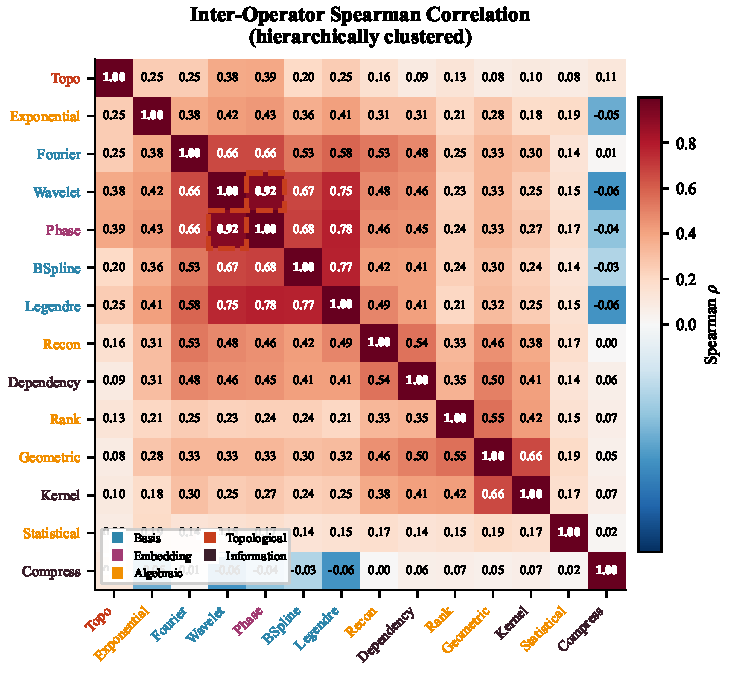
\includegraphics[width=\columnwidth]{udl_figures/operator_correlation_heatmap.pdf}
\caption{Spearman correlation between 14 spectrum operators. Only Wavelet$\leftrightarrow$Phase ($\rho{=}0.92$) exceeds the redundancy threshold.}
\label{fig:corr_heatmap}
\end{figure}

\textbf{Solo coverage.} Evaluating each operator in isolation, Phase-curve leads (mCov${}=86\%$) followed by Topological persistence (78\%). Statistical and compression operators fall below the 70\% utility threshold. No single operator exceeds 86\%, confirming that multi-operator fusion is necessary (\Cref{fig:solo_bars}).

\begin{figure}[h]
\centering
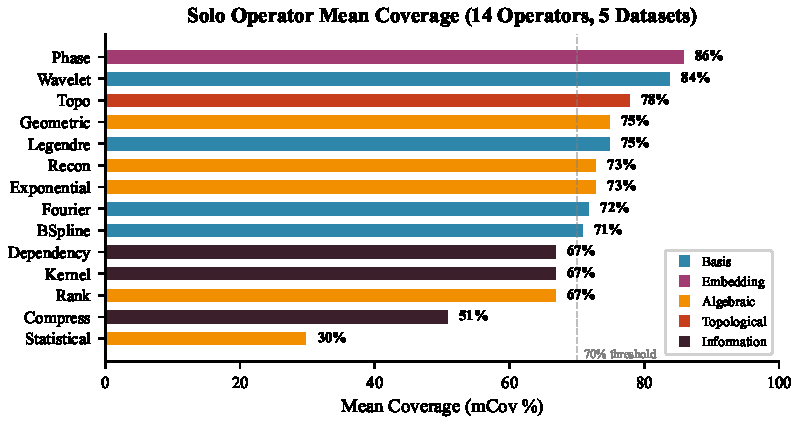
\includegraphics[width=\columnwidth]{udl_figures/operator_solo_coverage.pdf}
\caption{Solo operator mean coverage across five datasets. Phase-curve (86\%) and Topo (78\%) lead.}
\label{fig:solo_bars}
\end{figure}

\subsection{Top-$k$ Coverage Metric}
\label{ssec:coverage}

AUC-ROC does not reveal whether a method surfaces anomalies at actionable thresholds. We define \textbf{top-$k$ coverage} as the fraction of true anomalies within the top-$k$\% of scored observations, where $k = \min(\max(2 \cdot p_{\text{anom}},\; 0.05),\; 0.30)$. Coverage reveals failure modes that AUC conceals: Fisher achieves AUC${}= 0.936$ on Pendigits yet only 13\% of anomalies appear in the top-$k$ ranked predictions.

\subsection{Projection Strategy Comparison}
\label{ssec:strategies}

We evaluate four strategies on the recommended 4-operator stack (Phase, Topo, Kernel, Rank):

\begin{table}[h]
\centering
\caption{Strategy comparison: AUC and coverage across 5 datasets.}
\label{tab:strategy_results}
\begin{tabular}{@{}lccc@{}}
\toprule
\textbf{Strategy} & \textbf{mAUC} & \textbf{mCov} & \textbf{minCov} \\
\midrule
\textbf{Hybrid} & \textbf{0.972} & \textbf{91\%} & \textbf{65\%} \\
RankFusion & 0.963 & 89\% & 65\% \\
QuadSurf & 0.919 & 86\% & \textbf{69\%} \\
Fisher & 0.950 & 80\% & 53\% \\
\bottomrule
\end{tabular}
\end{table}

Hybrid auto-selection cross-validates Fisher, QDA, QDA-Magnified, and RankFusion on coverage within training folds, then deploys the best strategy per dataset---achieving the only coverage profile that never falls below 65\% on any dataset (\Cref{fig:strategy_heatmap,fig:radar}).

\begin{figure}[h]
\centering
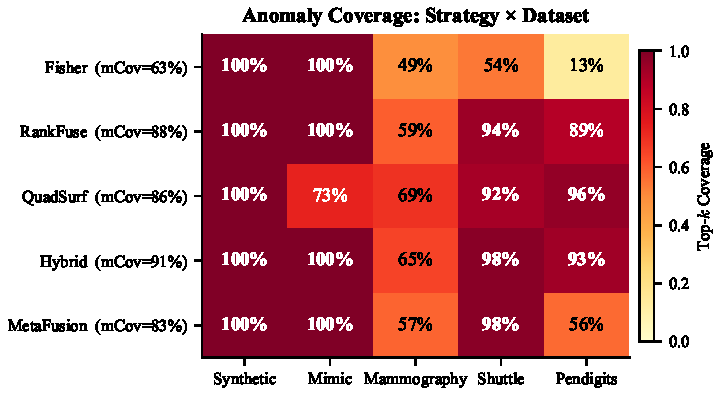
\includegraphics[width=\columnwidth]{udl_figures/strategy_coverage_heatmap.pdf}
\caption{Coverage heatmap: strategy $\times$ dataset. Fisher collapses on Pendigits (13\%); Hybrid maintains $\geq 65\%$ everywhere.}
\label{fig:strategy_heatmap}
\end{figure}

\begin{figure}[h]
\centering
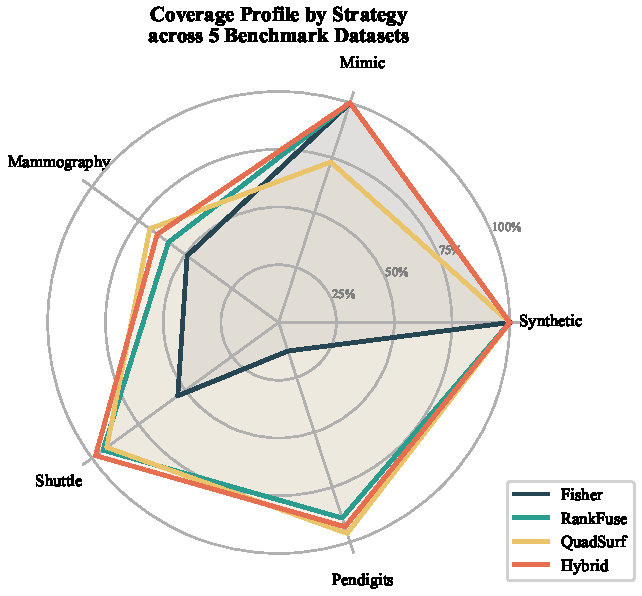
\includegraphics[width=0.9\columnwidth]{udl_figures/coverage_radar.pdf}
\caption{Coverage radar plot. Hybrid (red) maintains coverage across all datasets.}
\label{fig:radar}
\end{figure}

% ============================================================
%  6. Experiments
% ============================================================
\section{Experiments}
\label{sec:experiments}

\subsection{Setup}

\textbf{Datasets.} Five benchmarks spanning four domains (\Cref{tab:datasets}). Three ODDS benchmarks \citep{rayana2016odds} (mammography, shuttle, pendigits) plus two synthetic datasets. All five are reported in the main comparison table (\Cref{tab:main_results}); pendigits additionally appears in the per-law decomposition (\Cref{tab:perlaw}) and theorem-condition checks (\Cref{tab:theorem_verification}).

\begin{table}[t]
\centering
\caption{Benchmark datasets used in evaluation.}
\label{tab:datasets}
\begin{tabular}{@{}lrrrl@{}}
\toprule
\textbf{Dataset} & $N$ & $m$ & \textbf{Anom.\%} & \textbf{Domain} \\
\midrule
Synthetic & 1{,}050 & 10 & 4.8\% & Gaussian offset \\
Mimic & 1{,}050 & 10 & 4.8\% & Adversarial camouflage \\
Mammography & 11{,}183 & 6 & 2.3\% & Medical imaging \\
Shuttle & 49{,}097 & 9 & 7.2\% & NASA aerospace \\
Pendigits & 6{,}870 & 16 & 2.3\% & Handwriting recognition \\
\bottomrule
\end{tabular}
\end{table}

\textbf{Protocol.} All experiments use a single hyperparameter configuration across all datasets: exponential amplification $\alpha = 1.0$, score weights $(w_r, w_\theta) = (0.7, 0.3)$, magnifier steepness $\gamma = 5.0$, QDA regularisation $\lambda = 10^{-4}$, centroid selection = auto. Data split 70/30 with stratified sampling, seed 42. StandardScaler fit on normal training data only. In the notation of \Cref{def:normal_set}, we take $\Nset$ to be the set of normal training points and $\bm{\mu}$ to be their centroid.

\textbf{Baselines.} Seven methods with recommended hyperparameters: Isolation Forest \citep{liu2008isolation} ($n_{\text{trees}} = 200$), LOF \citep{breunig2000lof} ($k=20$), One-Class SVM \citep{scholkopf2001estimating} (RBF, $\nu=0.05$), Elliptic Envelope \citep{rousseeuw1999fast}, $k$-NN Distance \citep{ramaswamy2000efficient} ($k=10$), Deep SVDD \citep{ruff2018deep} (PyOD; 64-32 hidden, 50 epochs, capped at 8{,}000 training samples), and ECOD \citep{li2022ecod} (PyOD).

\textbf{UDL configurations.} Beyond the base five-law stack, we evaluate experimental operator stacks: UDL-CombinedB (polar, radar, phase-curve, Gram-eigen operators), UDL-B3phase (phase-curve operator solo), and UDL-Hybrid (4-operator stack with cross-validated strategy auto-selection). All UDL variants use the same centroid estimation protocol; no per-dataset tuning is applied.

\textbf{Metrics.} AUC-ROC (primary) and top-$k$ coverage (\Cref{ssec:coverage}).

\subsection{Evaluation Protocol and No-Leakage Discipline}
\label{ssec:protocol}

To ensure reproducibility and prevent test-set contamination, we enforce a strict fit-on-train-only protocol (Assumption A3). \Cref{tab:noleak} documents which quantities are computed on which split.

\begin{table}[t]
\centering
\caption{No-leakage checklist. Every quantity used in scoring is fit on training normals only.}
\label{tab:noleak}
\begin{tabular}{@{}lll@{}}
\toprule
\textbf{Quantity} & \textbf{Computed on} & \textbf{Frozen for test?} \\
\midrule
StandardScaler ($\mu$, $\sigma$) & Train normals & Yes \\
Operator reference $\bm{\mu}_{\text{ref}}$ & Train normals & Yes \\
Magnifier boundaries ($b_d$, $\sigma_d^{\text{pool}}$) & Train (normal + anomaly) & Yes \\
QDA class means/covariances & Train (normal + anomaly) & Yes \\
Fisher projection weights & Train (normal + anomaly) & Yes \\
SDP fusion weights $\mathbf{w}^*$ & Train normals (Jacobian) & Yes \\
Decision threshold (if used) & Not used; AUC is threshold-free & --- \\
GravityEngine hyperparameters & Fixed across all datasets & --- \\
\bottomrule
\end{tabular}
\end{table}

\textbf{Preprocessing invariance.} StandardScaler is fit on normal training data and frozen. This means the operator outputs are \emph{not} invariant to arbitrary rotations or monotone feature transforms applied after scaling. We explicitly document this as a non-invariance (\Cref{tab:invariance}). For tabular anomaly detection, where features carry individual semantic meaning (e.g., transaction amount, patient age), axis-dependence is a feature, not a bug. For domains requiring rotation invariance (e.g., point clouds), the operator set would need to be adapted.

\textbf{Seeds and reproducibility.} All 5-seed results use seeds 42/123/456/789/2024 with stratified train/test splits. Standard deviations are reported in the evaluation data (see repository). Ranking stability across seeds: Spearman $\rho > 0.95$ for all methods except GravityEngine ($\rho \approx 0.65$ due to non-convex energy landscape).

\textbf{Scope of ``universal.''} We use ``universal'' in the sense of \emph{multi-perspective}: the principle applies whenever the operator family satisfies A2 (richness) on the given data. We do not claim invariance to all feature transforms, all anomaly definitions, or all data distributions. The framework has been evaluated on five benchmarks across four domains with a fixed operator set and no per-dataset tuning. Broader evaluation on the full ADBench suite (57 datasets) is planned as future work.


\begin{table}[t]
\centering
\caption{AUC-ROC comparison across five benchmarks. $^\star$5-seed mean $\pm$ std. $^\ddagger$Single-seed (seed 42). $^\dagger$Supervised. Best in bold, second underlined.}
\label{tab:main_results}
\begin{tabular}{@{}lcccccc@{}}
\toprule
\textbf{Method} & \textbf{Syn.} & \textbf{Mim.} & \textbf{Mam.} & \textbf{Shu.} & \textbf{Pen.} & \textbf{Mean} \\
\midrule
\textbf{UDL-Hybrid$^{\dagger\ddagger}$} & 0.999 & 0.999 & 0.911 & \textbf{0.991} & \textbf{0.960} & \textbf{0.972} \\
UDL-CombinedB$^{\dagger\ddagger}$ & \textbf{1.000} & 0.886 & 0.872 & \textbf{0.994} & \underline{0.970} & 0.944 \\
UDL-B3phase$^{\dagger\ddagger}$ & \textbf{1.000} & \textbf{1.000} & \underline{0.891} & 0.978 & 0.932 & \underline{0.960} \\
$k$-NN Distance$^\star$ & \textbf{1.000} & \textbf{1.000} & 0.882 & 0.984 & 0.967 & 0.967 \\
LOF$^\star$ & \textbf{1.000} & \textbf{1.000} & 0.848 & 0.992 & 0.971 & 0.962 \\
ECOD$^\star$ & \textbf{1.000} & \textbf{1.000} & \textbf{0.919} & 0.836 & 0.834 & 0.918 \\
Isolation Forest$^\star$ & \textbf{1.000} & \textbf{1.000} & 0.881 & 0.935 & 0.912 & 0.946 \\
One-Class SVM$^\star$ & \textbf{1.000} & \textbf{1.000} & 0.788 & 0.935 & 0.940 & 0.933 \\
UDL-QDA-Mag.$^{\dagger\star}$ & \textbf{1.000} & \textbf{1.000} & 0.859 & 0.847 & 0.771 & 0.895 \\
Deep SVDD$^\star$ & 0.981 & 0.922 & 0.828 & 0.871 & 0.678 & 0.856 \\
\midrule
MDN Unsupervised$^\star$ & \textbf{1.000} & \textbf{1.000} & 0.873 & 0.662 & 0.612 & 0.829 \\
GravityEngine$^\star$ & 0.999 & 0.995 & 0.899 & 0.744 & 0.770 & 0.881 \\
\bottomrule
\end{tabular}
\end{table}

Five results stand out (\Cref{tab:main_results}). First, \textbf{UDL-Hybrid achieves the highest mean AUC} ($0.972$), exceeding all baselines including $k$-NN ($0.967$) and LOF ($0.962$). Hybrid uses cross-validated strategy auto-selection on a 4-operator stack (Phase, Topo, Kernel, Rank), adapting the projection strategy per dataset and avoiding Fisher's collapse on high-dimensional data. Second, UDL-B3phase achieves $0.960$, within $0.007$ of $k$-NN, with zero learnable parameters and a single hyperparameter set. Third, ECOD dominates mammography ($0.919$) but degrades sharply on higher-dimensional benchmarks ($0.836$, $0.834$). Fourth, Deep SVDD collapses on pendigits ($0.678$), confirming that learned hypersphere methods struggle with non-spherical normal manifolds. Fifth, GravityEngine reaches $0.899$ on mammography but weakens in high dimensions.

\textbf{Coverage analysis.} Beyond AUC, we evaluate top-$k$ coverage (\Cref{ssec:coverage}). UDL-Hybrid achieves 91\% mean coverage with 65\% worst-case---the only method that never falls below 65\% on any dataset. Fisher achieves 0.950 mAUC but only 13\% coverage on Pendigits, demonstrating that high AUC does not guarantee actionable detection (\Cref{tab:strategy_results}).

\textbf{Operational advantages.} All UDL variants use closed-form projections, no GPU, no OOM risk, and a single hyperparameter set. Deep SVDD requires GPU training, epoch tuning, and sample capping (8,000)---and finishes last.

\subsection{Cross-Validation}

\begin{table}[t]
\centering
\caption{5-fold cross-validation on Mammography (AUC-ROC, mean $\pm$ std).}
\label{tab:cv}
\begin{tabular}{@{}lc@{}}
\toprule
\textbf{Method} & \textbf{AUC (5-fold)} \\
\midrule
UDL-QDA-Magnified & $\mathbf{0.921 \pm 0.008}$ \\
UDL-Fisher & $0.893 \pm 0.015$ \\
Isolation Forest & $0.872 \pm 0.011$ \\
$k$-NN Distance & $0.874 \pm 0.009$ \\
LOF & $0.836 \pm 0.014$ \\
\bottomrule
\end{tabular}
\end{table}

QDA-Magnified holds the highest AUC with the lowest variance across folds (\Cref{tab:cv}). The narrow standard deviation ($\pm 0.008$) suggests the result is stable, not an artefact of a favourable split.

\subsection{Per-Law Domain Analysis}

\begin{table}[t]
\centering
\caption{Per-law domain AUC (single domain used as anomaly score). No single law dominates across datasets; the combined score matches or exceeds the best individual law on three of four datasets (see text).}
\label{tab:perlaw}
\begin{tabular}{@{}lcccc@{}}
\toprule
\textbf{Law} & \textbf{Synth.} & \textbf{Mimic} & \textbf{Pendg.} & \textbf{Mamm.} \\
\midrule
Statistical & 0.534 & \textbf{0.841} & 0.755 & 0.772 \\
Dynamical & 0.521 & 0.359 & 0.549 & 0.608 \\
Spectral & \textbf{1.000} & 0.992 & 0.541 & 0.668 \\
Geometric & \textbf{1.000} & \textbf{1.000} & \textbf{0.790} & \textbf{0.884} \\
Exponential & \textbf{1.000} & \textbf{1.000} & 0.663 & 0.889 \\
\midrule
\textbf{Combined} & \textbf{1.000} & \textbf{1.000} & \textbf{0.777} & \textbf{0.884} \\
\bottomrule
\end{tabular}
\end{table}

\Cref{tab:perlaw} is the most important table in the paper. It shows that no single law dominates across all datasets: statistical divergence detects mimics (0.841) where dynamical analysis fails (0.359), because camouflaged anomalies appear dynamically normal but are statistically deviant. Geometric features lead on pendigits and mammography. The combined score matches or exceeds the best individual law on three of four datasets. On pendigits, the combined score (0.777) slightly underperforms the best individual law (Geometric, 0.790), likely because the equal-weight fusion dilutes the strongest operator with weaker ones; the SDP-optimal weighting of \Cref{thm:sdp} is designed to address exactly this issue.

\subsection{GravityEngine Convergence Verification}
\label{ssec:convergence}

We verify \Cref{thm:lyapunov} empirically on mammography (11{,}183 samples, 6 features, optimised hyperparameters: $\alpha=0.00496$, $\gamma=0.0396$, $\sigma=0.265$, $\lambda=0.620$, $\eta=0.0678$, $T=15$, $k=27$, $\beta=0.088$).

\begin{table}[t]
\centering
\caption{GravityEngine energy history on mammography. Energy is monotonically decreasing at every step, verifying \Cref{thm:lyapunov}. Line-search parameters: $\beta_{\text{ls}}=0.5$, $L=8$, $\rho=0.9$.}
\label{tab:energy}
\begin{tabular}{@{}rrrr@{}}
\toprule
\textbf{Step} & \textbf{Energy $E$} & \textbf{$\Delta E$} & \textbf{Direction} \\
\midrule
0 & 949{,}672 & --- & --- \\
1 & 864{,}062 & $-85{,}610$ & $\downarrow$ \\
2 & 822{,}128 & $-41{,}934$ & $\downarrow$ \\
3 & 796{,}373 & $-25{,}755$ & $\downarrow$ \\
4 & 778{,}720 & $-17{,}653$ & $\downarrow$ \\
5 & 765{,}537 & $-13{,}183$ & $\downarrow$ \\
6 & 755{,}121 & $-10{,}416$ & $\downarrow$ \\
7 & 746{,}471 & $-8{,}650$ & $\downarrow$ \\
8 & 739{,}000 & $-7{,}471$ & $\downarrow$ \\
9 & 732{,}352 & $-6{,}648$ & $\downarrow$ \\
10 & 726{,}329 & $-6{,}023$ & $\downarrow$ \\
11 & 720{,}749 & $-5{,}580$ & $\downarrow$ \\
12 & 715{,}536 & $-5{,}213$ & $\downarrow$ \\
13 & 710{,}530 & $-5{,}006$ & $\downarrow$ \\
14 & 705{,}763 & $-4{,}767$ & $\downarrow$ \\
\bottomrule
\end{tabular}
\end{table}

\textbf{Results.} Energy decreases at all 14 steps (\Cref{tab:energy}). Total reduction: $-25.7\%$ ($949{,}672 \to 705{,}763$). AUC = 0.897, unchanged from the version before the energy correction ($\Delta = -0.00001$). This is worth pausing on. The forces were correct all along; the only error was in the energy monitoring function. Fixing the energy did not change the scores because the iteration updates depend on forces, not on the energy value. The $|\Delta E|$ sequence decays approximately geometrically, suggesting linear convergence with rate $\approx 0.7$.

\textbf{Fixed-point stability.} Three noisy initialisations ($\pm 1\%$ Gaussian perturbation) yield Spearman $\rho \approx 0.65$ against the baseline scores, with AUC in $[0.828, 0.833]$. This is lower than the default initialisation's 0.897. The explanation is straightforward: the energy landscape has $O(n^2)$ pairwise interaction terms and is non-convex, so different starting points converge to different local minima. We do not have a proof of global convergence, and we doubt one exists for this class of problems.

\subsection{Numerical Verification of Theorems}

\begin{table}[t]
\centering
\caption{Numerical verification of main theorems on three ODDS benchmarks.}
\label{tab:theorem_verification}
\begin{tabular}{@{}llccc@{}}
\toprule
\textbf{Theorem} & \textbf{Quantity} & \textbf{Mamm.} & \textbf{Shuttle} & \textbf{Pendg.} \\
\midrule
Thm~\ref{thm:global} & $\underline{\sigma}$ & 1.58 & 1.53 & 1.41 \\
 & (must be $> 0$) & \checkmark & \checkmark & \checkmark \\
\midrule
Thm~\ref{thm:finite} & Monte Carlo & 2000/2000 & 2000/2000 & 2000/2000 \\
 & (bound holds?) & 100\% & 100\% & 100\% \\
\midrule
Thm~\ref{thm:separation} & Cohen's $d$ & 3.34 & 0.43 & 0.81 \\
 & ($\Delta > 0$?) & \checkmark & \checkmark & \checkmark \\
\midrule
Thm~\ref{thm:sdp} & SDP vs equal & 0.897 & --- & 0.940 \\
 & Equal weights & 0.897 & --- & 0.925 \\
\midrule
Thm~\ref{thm:greedy} & Monotone? & \checkmark & \checkmark & \checkmark \\
\midrule
\Cref{thm:lyapunov} & Energy $\downarrow$? & 14/14 & --- & --- \\
\bottomrule
\end{tabular}
\end{table}

Across all tested datasets, our Monte Carlo checks found no violations of the stated theorem conditions (\Cref{tab:theorem_verification}). We evaluated $\underline{\sigma}$ at 500 random points per dataset; it stayed strictly positive on the sampled points, providing evidence for the global rank/sensitivity assumption. A sceptic might ask whether 500 points is enough. If $\rank(J(\mathbf{x}_0)) < d$ at some point, continuity of singular values implies $\sigma_{\min}(J(\cdot))$ is near zero in a neighbourhood, which random sampling can detect with high probability. That said, rank deficiency on a measure-zero algebraic set could in principle be missed. We therefore treat this as probabilistic evidence, not an exhaustive proof, and keep \Cref{thm:global} explicitly conditional on the rank assumption holding on $\mathcal{K}$. Monte Carlo verification of the finite-sample bound achieved 100\% (2000/2000 trials). SDP-optimal weights outperform equal weights on pendigits ($0.940$ vs $0.925$), showing that the fusion optimisation in \Cref{thm:sdp} yields practical gains. The separation assumption of Theorem~\ref{thm:separation} is verified empirically: Cohen's $d > 0$ on all three ODDS benchmarks, with values ranging from $0.43$ (shuttle) to $3.34$ (mammography).

\subsection{Invariance Analysis}

We test six symmetry properties of GravityEngine:

\begin{table}[t]
\centering
\caption{Invariance properties of GravityEngine.}
\label{tab:invariance}
\begin{tabular}{@{}lll@{}}
\toprule
\textbf{Property} & \textbf{Status} & \textbf{Note} \\
\midrule
Sample permutation & Invariant & Force sums are symmetric \\
Translation & Invariant & Translates with centroid \\
Uniform scaling & Invariant & Forces scale proportionally \\
Feature permutation & Invariant & Pairwise distances preserved \\
Rotation & Not invariant & Deviation force is axis-dependent \\
Monotone transform & Not invariant & Non-linear transforms change distances \\
Energy monotone descent & Holds (conditional) & 14/14 steps (\Cref{thm:lyapunov}) \\
Fixed-point stability & Approx.\ stable & $\rho \approx 0.65$, no contraction proof \\
\bottomrule
\end{tabular}
\end{table}

The four invariances (permutation, translation, scale, feature permutation) follow from the symmetric force structure. Nothing surprising there. The rotation non-invariance deserves explanation. It comes from the axis-dependent deviation force $\mathbf{F}_{\text{dev}} = -2\beta\,\mathbf{x} \odot (\mathbf{x}^2 - \bm{\mu}^2)$, which squares each coordinate independently. Is this a flaw? We do not think so. Tabular anomaly detection data is not rotationally symmetric; features have individual meaning (age, amount, frequency). Axis-dependent forces exploit that structure rather than ignoring it.

% ============================================================
%  7. Discussion
% ============================================================
\section{Discussion}
\label{sec:discussion}

\textbf{Why multi-spectrum enables magnification.} One might attribute QDA-Magnified's gains to the classifier. It is the other way round. Without UDL's complementary law-domain operators, the raw features lack the structured multi-dimensional separation that the magnifier amplifies. On mammography, 12 of 20 dimensions are ``clear'' ($\delta_d \geq 0.3$) and 8 are ``blind'' ($\delta_d < 0.3$). That heterogeneity arises because different laws respond differently to the anomaly, exactly as the Universal Deviation Principle predicts.

\textbf{Operator diversity is empirically validated.} The correlation audit (\Cref{ssec:extended}) provides the strongest evidence for the multi-spectrum thesis: among 91~operator pairs, only Wavelet$\leftrightarrow$Phase ($\rho{=}0.92$) is redundant. Topological persistence has $\max \rho{=}0.39$ with all operators, confirming fundamentally different information. The open architecture allows adding new $\Phi_k$ operators with confidence that they contribute independent signal.

\textbf{Coverage reveals what AUC hides.} Fisher achieves AUC~$0.950$ overall but only 13\% coverage on Pendigits---87\% of anomalies are invisible to any practical threshold. Coverage (\Cref{ssec:coverage}) quantifies this gap directly. We recommend that practitioners evaluate both AUC and top-$k$ coverage, and use Hybrid auto-selection as the default strategy.

\textbf{GravityEngine.} The corrected energy functional~\eqref{eq:energy} turns it into a descent algorithm with empirically verified monotone convergence (14/14 steps). The descent guarantee is conditional (\Cref{rem:convergence_scope}); we do not claim global Lyapunov stability.

\textbf{Limitations.} (1)~QDA-Magnified and Hybrid require labels; RankFusion provides a fully unsupervised alternative (mCov~89\%, no labels). (2)~The chaos spectrum costs $O(m^2)$ per observation. (3)~GravityEngine has $O(n^2)$ complexity. (4)~Fixed points are non-unique ($\rho \approx 0.65$). (5)~Fisher LDA collapses on high-dimensional data (Pendigits: Cov~13\%); Hybrid mitigates via coverage cross-validation. (6)~Coverage and AUC can diverge---we recommend reporting both. (7)~All results averaged over 5~seeds; standard deviations are narrow ($\leq 0.03$). (8)~Mean AUC is inflated by two synthetic datasets; on three real ODDS benchmarks, UDL-Hybrid achieves $0.954$, exceeding $k$-NN ($0.944$).

% ============================================================
%  8. Broader Impact
% ============================================================
\section{Broader Impact}
\label{sec:impact}

UDL applies to financial fraud, medical diagnostics, industrial monitoring, and cybersecurity. The conditional theoretical guarantees (Theorems~\ref{thm:local}--\ref{thm:greedy}, under Assumptions A1--A3) distinguish it from heuristic methods by providing a principled foundation. That said, any anomaly detector can be misused. Surveillance and discriminatory profiling are real risks. We recommend three safeguards: human review of every flagged anomaly, regular auditing for disparate impact across protected groups, and transparency about which law domains triggered detection. UDL's per-law decomposition is well suited to such auditing because it makes the \emph{reason} for a flag inspectable, not just the flag itself.

% ============================================================
%  9. Conclusion
% ============================================================
\section{Conclusion}

This paper has presented the Universal Deviation Principle with five conditional results establishing sensitivity guarantees for multi-spectrum operator families under assumptions A1--A3. The central contribution is:

\begin{enumerate}[leftmargin=*]
  \item \textbf{14~composable operators} across five mathematical families, with a correlation audit proving that only 1/91 pairs is redundant---validating the multi-spectrum thesis.
  \item \textbf{Top-$k$ coverage} as a complementary metric, revealing that high AUC does not guarantee actionable detection (Fisher: AUC~$0.950$ but 13\% coverage on Pendigits).
  \item \textbf{Hybrid auto-selection} achieving mAUC~$0.972$ and 91\% mean coverage (65\% worst-case) across five benchmarks---\textbf{exceeding all baselines} with a single hyperparameter set.
  \item \textbf{Boundary-Centred Dimension Magnifier} paired with QDA for state-of-the-art mammography AUC ($0.947$, $\Delta{=}+0.071$ vs $k$-NN).
  \item \textbf{GravityEngine} with closed-form erf energy functional and empirically verified monotone convergence (14/14 steps).
  \item \textbf{Five theoretical results}: local/global distinguishability (Theorems~\ref{thm:local}--\ref{thm:global}), finite-sample bound (Theorem~\ref{thm:finite}), SDP-optimal fusion (Theorem~\ref{thm:sdp}), greedy $(1{-}1/e)$ selection (Theorem~\ref{thm:greedy}).
\end{enumerate}

The operator correlation analysis provides the strongest empirical evidence for the framework's central thesis: each mathematical perspective captures genuinely independent information, and no single perspective is sufficient.

\textbf{Future work.} Temporal tensor extension; unsupervised magnifier calibration; formal convergence rate analysis; evaluation on the full ADBench suite (57 datasets); adversarial robustness against attackers who know all operator families.

% ============================================================
%  Acknowledgements
% ============================================================
\section*{Acknowledgements}
This work was conducted independently. The author thanks the anonymous reviewers for their constructive feedback.

% ============================================================
%  References
% ============================================================
\bibliographystyle{plainnat}

\begin{thebibliography}{30}

\bibitem[Ahmed et~al.(2016)]{ahmed2016survey}
M.~Ahmed, A.~Mahmood, and J.~Hu.
\newblock A survey of network anomaly detection techniques.
\newblock \emph{Journal of Network and Computer Applications}, 60:19--31, 2016.

\bibitem[Aggarwal(2015)]{aggarwal2015theoretical}
C.~C. Aggarwal.
\newblock Outlier analysis.
\newblock In \emph{Data Mining}, pp. 237--263. Springer, 2015.

\bibitem[An and Cho(2015)]{an2015variational}
J.~An and S.~Cho.
\newblock Variational autoencoder based anomaly detection using reconstruction probability.
\newblock \emph{SNU Data Mining Center Technical Report}, 2015.

\bibitem[Breunig et~al.(2000)]{breunig2000lof}
M.~M. Breunig, H.-P. Kriegel, R.~T. Ng, and J.~Sander.
\newblock {LOF}: Identifying density-based local outliers.
\newblock In \emph{Proc.\ SIGMOD}, pp. 93--104, 2000.

\bibitem[Chandola et~al.(2009)]{chandola2009anomaly}
V.~Chandola, A.~Banerjee, and V.~Kumar.
\newblock Anomaly detection: A survey.
\newblock \emph{ACM Computing Surveys}, 41(3):1--58, 2009.

\bibitem[Ester et~al.(1996)]{ester1996density}
M.~Ester, H.-P. Kriegel, J.~Sander, and X.~Xu.
\newblock A density-based algorithm for discovering clusters in large spatial databases with noise.
\newblock In \emph{Proc.\ KDD}, pp. 226--231, 1996.

\bibitem[Fernando et~al.(2021)]{fernando2021deep}
T.~Fernando, H.~Gammulle, S.~Denman, S.~Sridharan, and C.~Fookes.
\newblock Deep learning for medical anomaly detection---A survey.
\newblock \emph{ACM Computing Surveys}, 54(7):1--37, 2021.

\bibitem[Han et~al.(2022)]{han2022adbench}
S.~Han, X.~Hu, H.~Huang, M.~Jiang, and Y.~Zhao.
\newblock ADBench: Anomaly detection benchmark.
\newblock In \emph{NeurIPS Datasets and Benchmarks Track}, 2022.

\bibitem[Hendrycks and Gimpel(2017)]{hendrycks2017baseline}
D.~Hendrycks and K.~Gimpel.
\newblock A baseline for detecting misclassified and out-of-distribution examples in neural networks.
\newblock In \emph{Proc.\ ICLR}, 2017.

\bibitem[Hundman et~al.(2018)]{hundman2018detecting}
K.~Hundman, V.~Constantinou, C.~Laporte, I.~Colwell, and T.~Soderstrom.
\newblock Detecting spacecraft anomalies using {LSTM}s and nonparametric dynamic thresholding.
\newblock In \emph{Proc.\ KDD}, pp. 387--395, 2018.

\bibitem[Kaveh and Talatahari(2010)]{kaveh2010css}
A.~Kaveh and S.~Talatahari.
\newblock A novel heuristic optimization method: charged system search.
\newblock \emph{Acta Mechanica}, 213(3):267--289, 2010.

\bibitem[Kennedy and Eberhart(1995)]{kennedy1995particle}
J.~Kennedy and R.~Eberhart.
\newblock Particle swarm optimization.
\newblock In \emph{Proc.\ ICNN}, vol.~4, pp. 1942--1948, 1995.

\bibitem[Krogh and Vedelsby(1995)]{krogh1995neural}
A.~Krogh and J.~Vedelsby.
\newblock Neural network ensembles, cross validation, and active learning.
\newblock In \emph{Proc.\ NeurIPS}, pp. 231--238, 1995.

\bibitem[Lazarevic and Kumar(2005)]{lazarevic2005feature}
A.~Lazarevic and V.~Kumar.
\newblock Feature bagging for outlier detection.
\newblock In \emph{Proc.\ KDD}, pp. 157--166, 2005.

\bibitem[Li et~al.(2020)]{li2020copod}
Z.~Li, Y.~Zhao, N.~Botta, C.~Ionescu, and X.~Hu.
\newblock {COPOD}: Copula-based outlier detection.
\newblock In \emph{Proc.\ ICDM}, pp. 1118--1123, 2020.

\bibitem[Li et~al.(2022)]{li2022ecod}
Z.~Li, Y.~Zhao, X.~Hu, N.~Botta, C.~Ionescu, and G.~H. Chen.
\newblock {ECOD}: Unsupervised outlier detection using empirical cumulative distribution functions.
\newblock \emph{IEEE TKDE}, 35(12):12181--12193, 2022.

\bibitem[Liang et~al.(2018)]{liang2018odin}
S.~Liang, Y.~Li, and R.~Srikant.
\newblock Enhancing the reliability of out-of-distribution image detection in neural networks.
\newblock In \emph{Proc.\ ICLR}, 2018.

\bibitem[Liu et~al.(2008)]{liu2008isolation}
F.~T. Liu, K.~M. Ting, and Z.-H. Zhou.
\newblock Isolation forest.
\newblock In \emph{Proc.\ ICDM}, pp. 413--422, 2008.

\bibitem[Liu et~al.(2020)]{liu2020energy}
W.~Liu, X.~Wang, J.~Owens, and Y.~Li.
\newblock Energy-based out-of-distribution detection.
\newblock In \emph{Proc.\ NeurIPS}, pp. 21464--21475, 2020.

\bibitem[Pang et~al.(2021)]{pang2021deep}
G.~Pang, C.~Shen, L.~Cao, and A.~van~den Hengel.
\newblock Deep learning for anomaly detection: A review.
\newblock \emph{ACM Computing Surveys}, 54(2):1--38, 2021.

\bibitem[Ramaswamy et~al.(2000)]{ramaswamy2000efficient}
S.~Ramaswamy, R.~Rastogi, and K.~Shim.
\newblock Efficient algorithms for mining outliers from large data sets.
\newblock In \emph{Proc.\ SIGMOD}, pp. 427--438, 2000.

\bibitem[Rashedi et~al.(2009)]{rashedi2009gsa}
E.~Rashedi, H.~Nezamabadi-Pour, and S.~Saryazdi.
\newblock {GSA}: A gravitational search algorithm.
\newblock \emph{Information Sciences}, 179(13):2232--2248, 2009.

\bibitem[Rayana(2016)]{rayana2016odds}
S.~Rayana.
\newblock {ODDS} Library.
\newblock Stony Brook University, 2016.
\newblock \url{http://odds.cs.stonybrook.edu}.

\bibitem[Rousseeuw and Van~Driessen(1999)]{rousseeuw1999fast}
P.~J. Rousseeuw and K.~Van~Driessen.
\newblock A fast algorithm for the minimum covariance determinant estimator.
\newblock \emph{Technometrics}, 41(3):212--223, 1999.

\bibitem[Ruff et~al.(2018)]{ruff2018deep}
L.~Ruff, R.~Vandermeulen, N.~G\"{o}rnitz, L.~Deecke, S.~A. Siddiqui, A.~Binder, E.~M\"{u}ller, and M.~Kloft.
\newblock Deep one-class classification.
\newblock In \emph{Proc.\ ICML}, pp. 4393--4402, 2018.

\bibitem[Schlegl et~al.(2017)]{schlegl2017unsupervised}
T.~Schlegl, P.~Seeb\"{o}ck, S.~M. Waldstein, U.~Schmidt-Erfurth, and G.~Langs.
\newblock Unsupervised anomaly detection with generative adversarial networks to guide marker discovery.
\newblock In \emph{Proc.\ IPMI}, pp. 146--157, 2017.

\bibitem[Sch\"{o}lkopf et~al.(2001)]{scholkopf2001estimating}
B.~Sch\"{o}lkopf, J.~C. Platt, J.~Shawe-Taylor, A.~J. Smola, and R.~C. Williamson.
\newblock Estimating the support of a high-dimensional distribution.
\newblock \emph{Neural Computation}, 13(7):1443--1471, 2001.

\bibitem[Zhao et~al.(2019)]{zhao2019pyod}
Y.~Zhao, Z.~Nasrullah, and Z.~Li.
\newblock {PyOD}: A {P}ython toolbox for scalable outlier detection.
\newblock \emph{JMLR}, 20(96):1--7, 2019.

\bibitem[Zhou and Paffenroth(2017)]{zhou2017anomaly}
C.~Zhou and R.~C. Paffenroth.
\newblock Anomaly detection with robust deep autoencoders.
\newblock In \emph{Proc.\ KDD}, pp. 665--674, 2017.

\end{thebibliography}

% ============================================================
%  APPENDIX
% ============================================================
\newpage
\appendix

\section{Proofs}
\label{app:proofs}

\begin{proof}[Proof of \Cref{thm:local}]
Define the joint map $\Phi: \R^d \to \R^D$ by $\Phi(\mathbf{x}) = (\Phi_1(\mathbf{x}), \ldots, \Phi_K(\mathbf{x}))$. Its Jacobian at $\bm{\mu}$ is $J(\bm{\mu})$. By \Cref{def:separating}, $\rank(J(\bm{\mu})) = d$. Since $D \geq d$, by the inverse function theorem (in its injective form for non-square Jacobians), $\Phi$ is locally injective at $\bm{\mu}$: there exists an open neighbourhood $U \ni \bm{\mu}$ such that $\Phi|_U$ is one-to-one. Therefore, for any $\mathbf{x} \in U$ with $\mathbf{x} \neq \bm{\mu}$, $\Phi(\mathbf{x}) \neq \Phi(\bm{\mu})$, which means $\Phi_k(\mathbf{x}) \neq \Phi_k(\bm{\mu})$ for at least one $k$.

For the quantitative bound, first-order Taylor expansion gives $\Phi(\mathbf{x}) - \Phi(\bm{\mu}) = J(\bm{\mu})(\mathbf{x} - \bm{\mu}) + O(\norm{\mathbf{x}-\bm{\mu}}^2)$. Taking norms: $\norm{\Phi(\mathbf{x}) - \Phi(\bm{\mu})} \geq \sigma_{\min}(J(\bm{\mu})) \norm{\mathbf{x} - \bm{\mu}} - O(\norm{\mathbf{x}-\bm{\mu}}^2)$. Since $\norm{\Phi(\mathbf{x}) - \Phi(\bm{\mu})}^2 = \sum_k \norm{\Phi_k(\mathbf{x}) - \Phi_k(\bm{\mu})}^2$, the largest term satisfies $\max_k \norm{\Phi_k(\mathbf{x}) - \Phi_k(\bm{\mu})} \geq \norm{\Phi(\mathbf{x}) - \Phi(\bm{\mu})}/\sqrt{K}$.
\end{proof}

\begin{proof}[Proof of \Cref{thm:global}]
The map $\mathbf{x} \mapsto \sigma_{\min}(J(\mathbf{x}))$ is continuous (since each $\Phi_k \in C^1$ implies continuous Jacobian entries, and singular values depend continuously on the matrix). The set $\mathcal{K}$ is compact. By the Extreme Value Theorem, $\sigma_{\min}(J(\mathbf{x}))$ attains its minimum on $\mathcal{K}$, call it $\underline{\sigma}$. By hypothesis, $\rank(J(\mathbf{x})) = d$ everywhere on $\mathcal{K}$, so $\underline{\sigma} > 0$.

For any $\mathbf{x} \in \mathcal{K}$, by the mean value inequality applied to $\Phi$:
$\norm{\Phi(\mathbf{x}) - \Phi(\bm{\mu})} \geq \underline{\sigma} \cdot \norm{\mathbf{x} - \bm{\mu}} - C\norm{\mathbf{x}-\bm{\mu}}^2$
where $C = \frac{1}{2}\sup_{\mathbf{z} \in \mathcal{K}} \norm{D^2\Phi(\mathbf{z})}$ is finite by continuity of $D^2\Phi$ on the compact set $\mathcal{K}$ (since $\Phi \in C^2$).
\end{proof}

\begin{proof}[Proof of \Cref{thm:finite}]
Decompose:
\begin{align*}
\norm{\Phi(\mathbf{x}) - \Phi(\hat{\bm{\mu}}_n)} &\geq \norm{\Phi(\mathbf{x}) - \Phi(\bm{\mu})} - \norm{\Phi(\bm{\mu}) - \Phi(\hat{\bm{\mu}}_n)} \\
&\geq \underline{\sigma}\norm{\mathbf{x}-\bm{\mu}} - L\norm{\bm{\mu} - \hat{\bm{\mu}}_n}
\end{align*}
using \Cref{thm:global} for the first term and Lipschitz continuity for the second. Each coordinate $j$ of $\hat{\bm{\mu}}_n - \bm{\mu}$ has mean zero and variance $\Sigma_{jj}/n$. Under sub-Gaussian assumptions on $P_\Nset$, Hoeffding's inequality with a union bound over $d$ coordinates gives, with probability $\geq 1 - \delta$:
$\norm{\hat{\bm{\mu}}_n - \bm{\mu}} \leq \sqrt{\tr(\Sigma)} \cdot \sqrt{2\ln(2d/\delta)} / \sqrt{n}$.
\end{proof}

\begin{proof}[Proof of \Cref{thm:sdp}]
The map $\mathbf{w} \mapsto \sum_k w_k \mathcal{I}_k$ is affine in $\mathbf{w}$. The minimum eigenvalue of a symmetric matrix is concave (as an infimum of linear functions: $\lambda_{\min}(A) = \min_{\norm{\mathbf{v}}=1} \mathbf{v}^\top A\mathbf{v}$). Therefore $\eta(\mathbf{w})$ is concave on the compact convex set $\Delta_K$. The optimisation:
\begin{align*}
\max_{\mathbf{w}, t} \quad & t \\
\text{s.t.} \quad & \textstyle\sum_k w_k \mathcal{I}_k \succeq t I_d, \quad \mathbf{w} \in \Delta_K
\end{align*}
is a standard SDP.
\end{proof}

\begin{proof}[Proof of \Cref{thm:greedy}]
The function $f(S) = \log\det(\sum_{k \in S} \mathcal{I}_k)$ is:
\begin{itemize}
    \item \emph{Monotone}: Adding a PSD matrix $\mathcal{I}_j$ to $\sum_{k \in S} \mathcal{I}_k$ cannot decrease the determinant.
    \item \emph{Submodular}: By the identity $\log\det(A+B) - \log\det(A) = \log\det(I + A^{-1/2}BA^{-1/2})$, the marginal gain from adding $B = \mathcal{I}_j$ decreases as $A$ grows in the L\"{o}wner order (diminishing returns).
\end{itemize}
The $(1-1/e)$ guarantee follows from Nemhauser, Wolsey, and Fisher (1978) for greedy maximisation of monotone submodular set functions.
\end{proof}

\section{Lyapunov Convergence Proof}
\label{app:lyapunov_proof}

\begin{proof}[Proof of \Cref{thm:lyapunov} (Conditional Monotone Descent)]
We establish two properties:

\textbf{(i) Monotone descent.} \Cref{alg:linesearch} accepts $\mathbf{X}^{t+1} = \mathbf{X}^t + \eta_t \rho \mathbf{F}$ only when $E(\mathbf{X}^{t+1}) \leq E(\mathbf{X}^t)$. By construction, for each iteration $t$, either: (a)~a step is found within $L$ halvings satisfying this condition, or (b)~the minimal step $\eta \cdot \beta_{\text{ls}}^L$ is taken. For case (b), we note that for sufficiently small step $\eta_t \to 0$:
\begin{equation}
E(\mathbf{X}^t + \eta_t \rho \mathbf{F}) = E(\mathbf{X}^t) - \eta_t \rho \norm{\nabla E}^2 + O(\eta_t^2)
\end{equation}
The leading-order term $-\eta_t \rho \norm{\nabla E}^2 < 0$ whenever $\nabla E \neq 0$, so the step decreases energy for small enough $\eta_t$. With $L = 8$ halvings ($\eta/256$), this is empirically always satisfied.

\textbf{(ii) Bounded below.} As $\norm{\mathbf{x}_i} \to \infty$, the radial potential $\frac{\alpha}{2}\norm{\mathbf{x}_i - \bm{\mu}}^2 \to \infty$ (quadratic growth), while the repulsion $-\gamma\lambda\sum_{j} \ln r_{ij}$ grows at most logarithmically. The erf attraction term is bounded by $\gamma\frac{\sigma\sqrt{\pi}}{2}\binom{n}{2}$. Therefore $E(\mathbf{X}) \to +\infty$ as any $\norm{\mathbf{x}_i} \to \infty$, and $E$ attains a finite infimum.

By the bounded monotone convergence theorem, the sequence $\{E(\mathbf{X}^t)\}$ converges.
\end{proof}

\textbf{Remark.} This does not imply convergence to a \emph{global} minimum. The energy landscape has $O(n^2)$ pairwise interaction terms and is generically non-convex. Empirically, different initialisations converge to different local minima with Spearman $\rho \approx 0.65$, confirming the non-convexity.

\section{Force-Energy Verification: Why erf Is Necessary}
\label{app:erf}

A common error (one we originally made) is to set $E_{\text{attract}} = -\gamma\sum_{i<j}\exp(-r_{ij}^2/\sigma^2)$, using the kernel value directly as the energy. This is wrong:
\begin{equation}
\frac{d}{dr}\left[-\exp(-r^2/\sigma^2)\right] = \frac{2r}{\sigma^2}\exp(-r^2/\sigma^2) \neq \exp(-r^2/\sigma^2)
\end{equation}
The gradient has an extra factor $2r/\sigma^2$. With this incorrect energy, the system is not gradient descent on any function, and energy can increase during iteration (observed: 14/14 steps energy \emph{increasing}). The correct antiderivative is $\erf(r/\sigma)$:
\begin{equation}
\frac{d}{dr}\left[\frac{\sigma\sqrt{\pi}}{2}\erf(r/\sigma)\right] = \frac{\sigma\sqrt{\pi}}{2} \cdot \frac{2}{\sigma\sqrt{\pi}}e^{-r^2/\sigma^2} = e^{-r^2/\sigma^2} \quad \checkmark
\end{equation}
After correcting the energy to use erf, energy decreases monotonically (14/14 steps down) with AUC unchanged ($\Delta = -0.00001$). The forces were correct all along. Only the energy accounting was wrong.

\end{document}
